\documentclass{beamer}

\mode<presentation> {
	\usetheme{Madrid}
	%\setbeamertemplate{footline}
}

\usepackage{gensymb}
\usepackage[utf8]{inputenc}
\usepackage[russian]{babel}
\usepackage{graphicx} % Allows including images
\usepackage{booktabs} % Allows the use of \toprule, \midrule and \bottomrule in tables

\DeclareGraphicsExtensions{.jpg}

%----------------------------------------------------------------------------------------
%	Титульный лист
%----------------------------------------------------------------------------------------

\title{Leap Motion, карта глубин и OpenCV}

% \author{}
\institute[AIRLabs]
{
	
\includegraphics[scale=0.15]{AIRLab_logo}
	\medskip
}
\date{}

%----------------------------------------------------------------------------------------
%	Презентация
%----------------------------------------------------------------------------------------

\begin{document}

	\begin{frame}
		\titlepage
	\end{frame}

	\begin{frame}
		\frametitle{Обзор}
		\tableofcontents
	\end{frame}

	\section{Leap Motion}
		\begin{frame}
			\frametitle{Leap Motion}
			
			\begin{center}
				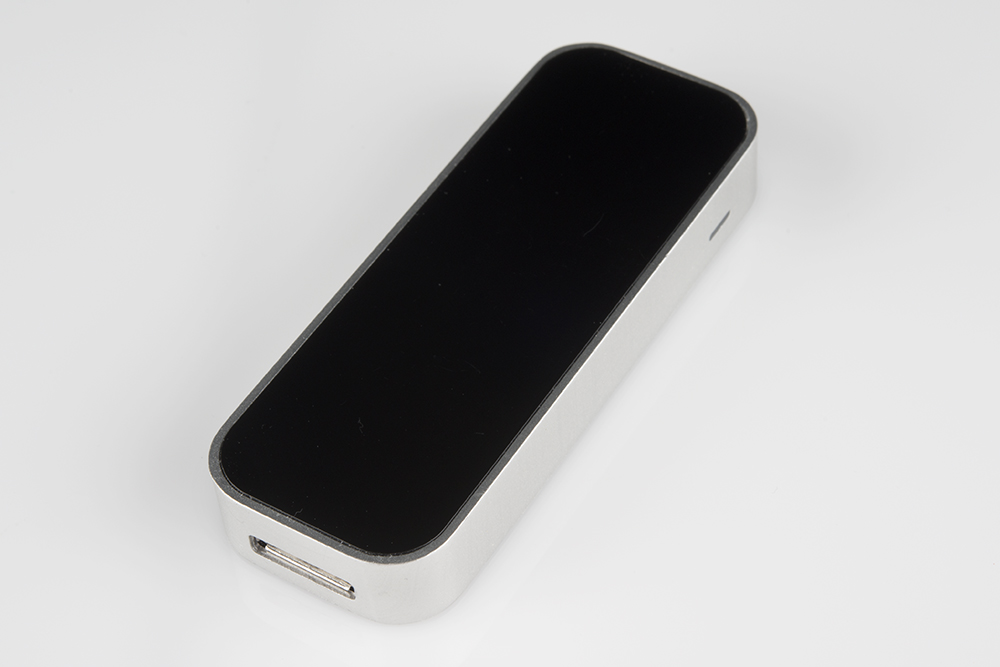
\includegraphics[scale=0.25]{LeapMotion}
			\end{center}
		\end{frame}
		
		\begin{frame}
			\frametitle{Особенности}
			
			\begin{itemize}
				\item 2 камеры с линзами fish-eye
				\item 3 инфракрасных светодиода
				\item Интерфейс: USB 3.0 micro-B
				\item Дальность распознавания объектов $\approx$ 60 см
				\item Угол обзора $\approx$ 135$\degree$
				\item Стандартный SDK умеет распознавать только руки
				\item Монохромные изображения с разрешением 620x240 на выходе
			\end{itemize}
			
			\begin{center}
				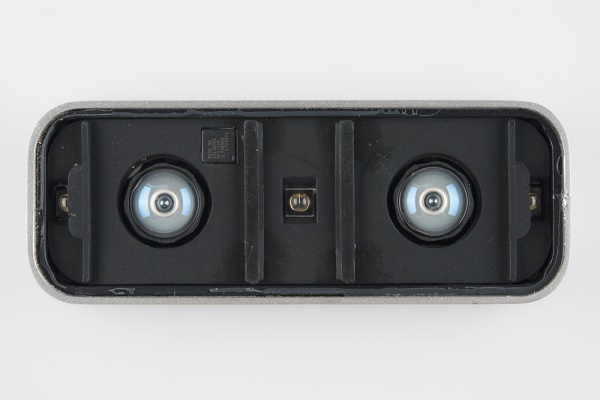
\includegraphics[scale=0.25]{LeapMotionDisassembled}
			\end{center}
		\end{frame}
		
		\begin{frame}
			\frametitle{Leap SDK}
			
			SDK позволяет делать множество интересных вещей:
			\begin{itemize}
				\item Определять руки, ладони, отдельные пальцы
				\item Определять инструменты (объекты цилиндрической формы вытянутые и тонкие)
				\item Определять жесты, такие как свайпы, нажатия и пр.
				\item Возвращать сырые изображения с камер
			\end{itemize}
		\end{frame}
		
		\begin{frame}
			\frametitle{Чем Leap Motion плох?}
			
			Цитата из интервью с одним из разработчиков:\\
			"... It’s very different from other things like the Kinect, and in normal device
			operation we have very different priorities than most other technologies.
			Our priority is precision, small movements, very low latency, very low CPU
			usage - so in order to do that we will often be making sacrifices that make
			what the device is doing completely not applicable to what I think you’re
			getting at, which is 3D scanning".
		\end{frame}
		
		\begin{frame}
			\frametitle{Чем Leap Motion плох?}
			
			Leap Motion не создает карту глубин, для распознавания рук применяются специальные
			алгоритмы. То есть, единственная информация, которая нас интересует - изображения.\\
			По сути, это просто две камеры.
		\end{frame}
		
		\begin{frame}
			\frametitle{Чем Leap Motion плох?}
				
			Хорошо, пусть так, тогда для получения карты глубин можно применить сторонние библиотеки,
			например OpenCV.\\
			Но и такой подход не дает нужного результата, так как:\\
			
			\begin{itemize}
				\item Камеры очень чувствительны к освещению
				\item Отражения света светодиодов распознаются как объекты
			\end{itemize}
			
			Из-за этих двух пунктов карта глубин получается зашумленной.
		\end{frame}
		
		\begin{frame}
			\frametitle{Чем Leap Motion плох?}
			
			К сожалению, эти недостатки были замечены поздно.\\
			Зато был отработан подход, который можно применить к любой другой
			системе объемного зрения.
		\end{frame}
		
	\section{Как мы творили темную магию объемного зрения}
		\begin{frame}
			\frametitle{Этапы}
			
			\begin{itemize}
				\item Калибровка
				\item Построение карты глубин (карты разностей/disparity map)
				\item Построение облака точек
				\item Blob detection
			\end{itemize}
		\end{frame}
		
		\begin{frame}
			\frametitle{Калибровка}
			В процессе производства камеры и линз всегда есть некоторые неточности, поэтому, всегда когда мы работаем со стереоскопией существует необходимость в калибровке: нахождении внешних и внутренних параметров стереопары.
		\end{frame}

		\begin{frame}
			\frametitle{Калибровка}
			Ниже представлена модель камеры-обскуры
			\begin{equation}
			s
			\begin{bmatrix}
			u\\v\\1
			\end{bmatrix}
			=
			\begin{bmatrix}
			f_{x}&0&c_{x}\\
			0&f_{y}&c_{y}\\
			0&0&1
			\end{bmatrix}
			\begin{bmatrix}
			r_{11}&r_{11}&r_{11}&t_{1}\\
			r_{21}&r_{22}&r_{23}&t_{2}\\
			r_{31}&r_{32}&r_{33}&t_{3}
			\end{bmatrix}
			\begin{bmatrix}
			X\\Y\\Z\\1
			\end{bmatrix}
			\end{equation}
		\end{frame}
		
		\begin{frame}
			\frametitle{Внутренние параметры}
			\begin{center}
			$
			\begin{bmatrix}
			f_{x}&0&c_{x}\\
			0&f_{y}&c_{y}\\
			0&0&1
			\end{bmatrix}
			$
			\end{center}
			$(f_{x},f_{y})$ - фокусное расстояние\\
			$(c_{x},c_{y})$ - координаты принципальной точки(точка пересечения плоскости изображения с оптической осью, совпадающая с центром фотографии. В реальных камерах, как правило, бывает немного смещена из-за оптических искажений)
		\end{frame}				
		\begin{frame}
			\frametitle{Внешние параметры}
			\begin{center}
			$
			\begin{bmatrix}
			r_{11}&r_{11}&r_{11}&t_{1}\\
			r_{21}&r_{22}&r_{23}&t_{2}\\
			r_{31}&r_{32}&r_{33}&t_{3}
			\end{bmatrix}
			$
			\end{center}
			Матрица для перехода из ситемы координат мира в систему координат камеры
		\end{frame}				
		\begin{frame}
			\frametitle{Другие переменные}
			$(X,Y,Z)$ - координаты исходной точки\\
			$(u,v)$ - координаты на изображении\\
			$s$ - переменная отвечающая за масштаб
		\end{frame}
		\begin{frame}
			\frametitle{Построение облака точек}
			
			Следующий этап - построить облако точек - это массив
			точек вида $(x, y, z)$ - координат относительно камеры, в
			этом помогает функция \textbf{ReprojectImageTo3D} из библиотеки
			OpenCV.\\
			Затем запоминаются $z$-компоненты при разных расстояниях от камеры
			и по полученным значениям интерполируем функцию зависимости
			расстояния до объекта от интенсивности цвета на карте глубин.
			
		\end{frame}
		
		\begin{frame}
			\frametitle{Blob detection}
			
			\textbf{Blob detection} - это нахождение регионов на изображении,
			которые отличаются по каким-то свойствам, вроде цвета
			или яркости, в сравнении с окружающими регионами.\\
			Грубо говоря, blob (капля) - это регион изображения,
			в котором какие-то свойства постоянны или почти
			постоянны.\\
			Все точки blob'а считаются в каком-то смысле
			одинаковыми.\\
			
		\end{frame}
		
		\begin{frame}
			\frametitle{Blob detection}
			
			Следующий этап - применить blob detection для карты глубин.\\
			С этой задачей вновь помог справиться OpenCV.\\
			Алгоритм, реализованный в OpenCV, таков:\\
			\begin{itemize}
				\item Конвертируем изображение "бинарное" изображение - только
					  из черного и белого цветов по заданным извне границам
				\item Извлекаем компоненты связности
				\item Группируем центры компонент - близкие компоненты относятся к одному blob'у
				\item По полученным группам получаем результирующую позицию blob'а
			\end{itemize}
			
		\end{frame}

\end{document} 